\section{通路分類モジュール}
通路分類モジュールについて述べる.
このモジュールは,シナリオの「条件」が満たされたかの判定に必要な
通路の特徴を,カメラ画像を入力として分類する.
使用するカメラについては,経路追従モジュールと同様に,データセットの収集時は3つ
学習後は1つである.
通路の特徴の分類は,島田らの手法に倣い,\ref{fig:class}に示す8つとしている.
% この中で,突き当たりは
% 行き止まり,角(右),角(左),三叉路(中央)
% 右手に通路が〜角(右)十字路 三叉路(右)三叉路(中央)
% 左手に通路が〜角(左)十字路 三叉路(中央)三叉路(左)
\begin{figure}[htbp]
    \centering
     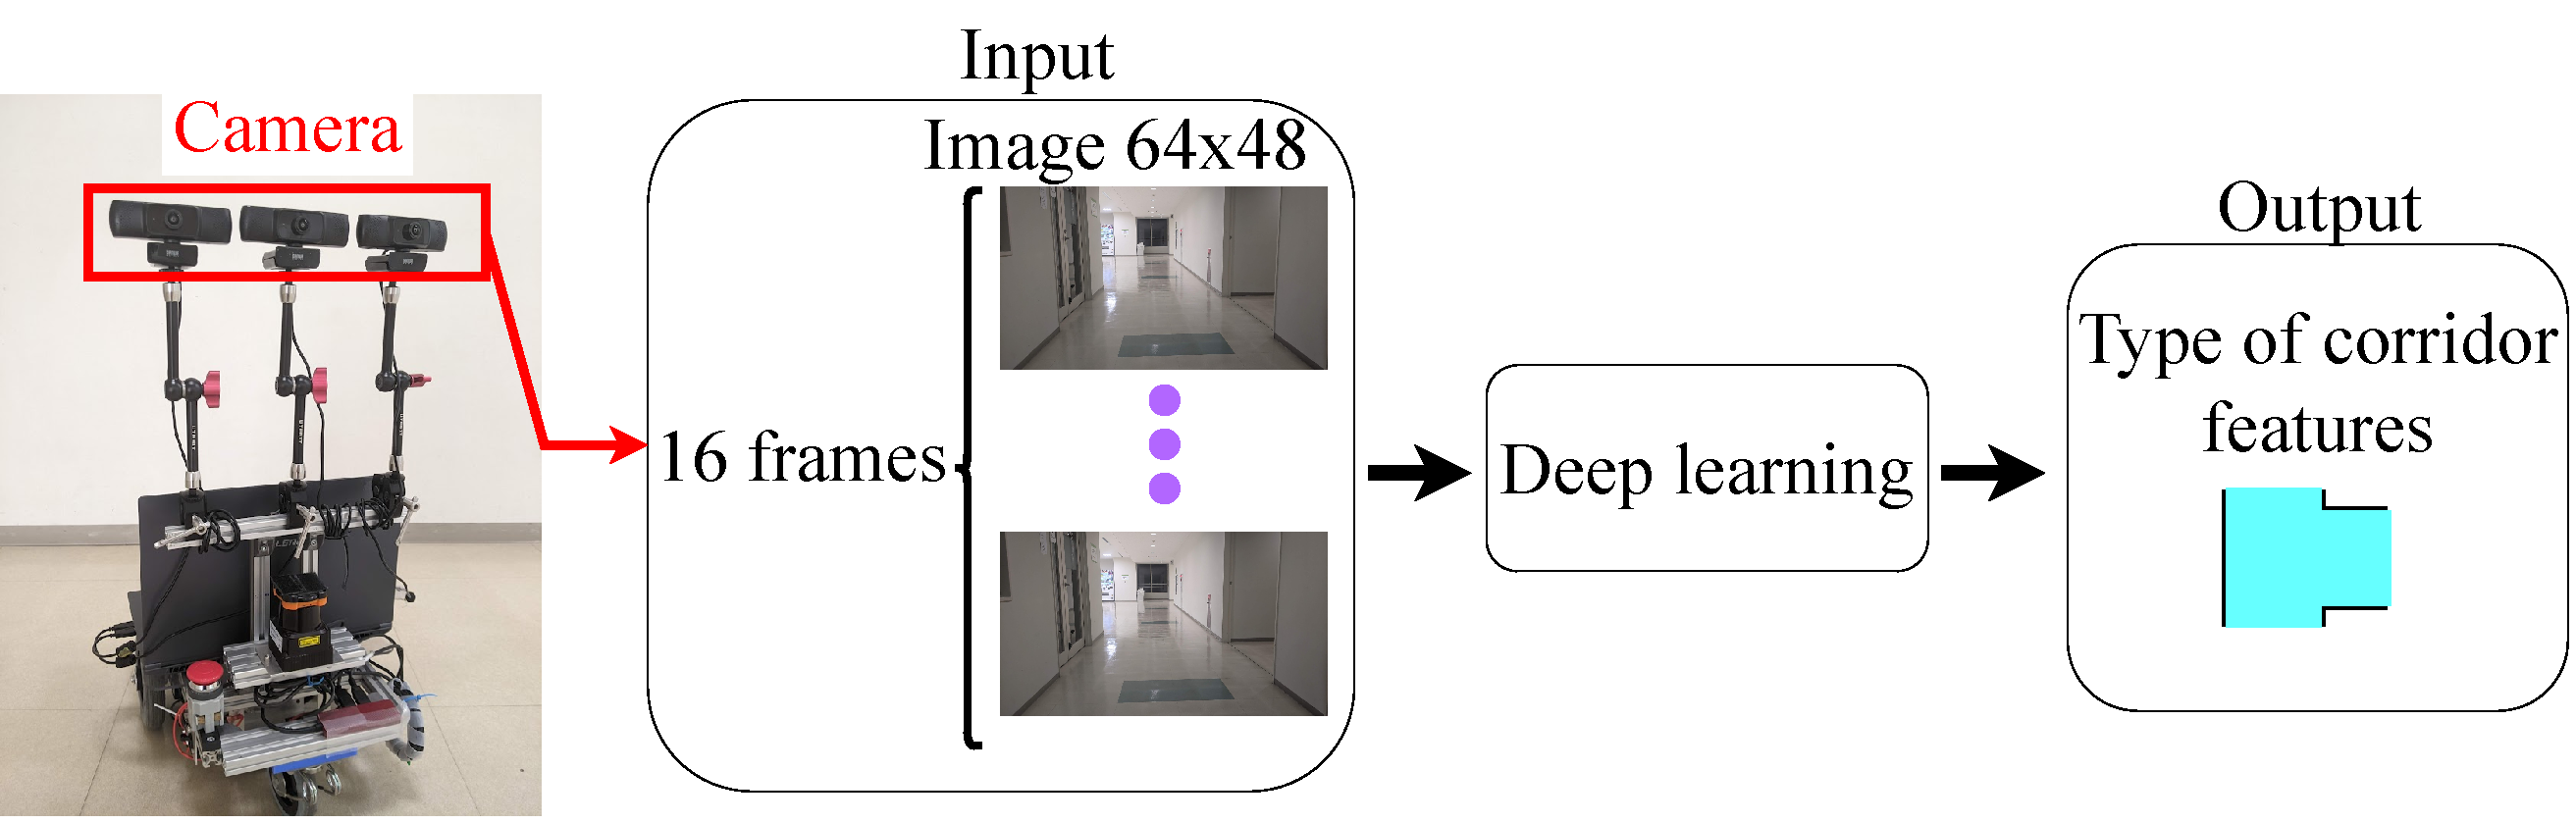
\includegraphics[width=100mm]{images/pdf/intersection_abs.pdf}
     \caption{Path-following module system Quoted from \cite{haruyama2023}}
     \label{fig:intersection_abs}
\end{figure}
\begin{figure}[htbp]
    \centering
     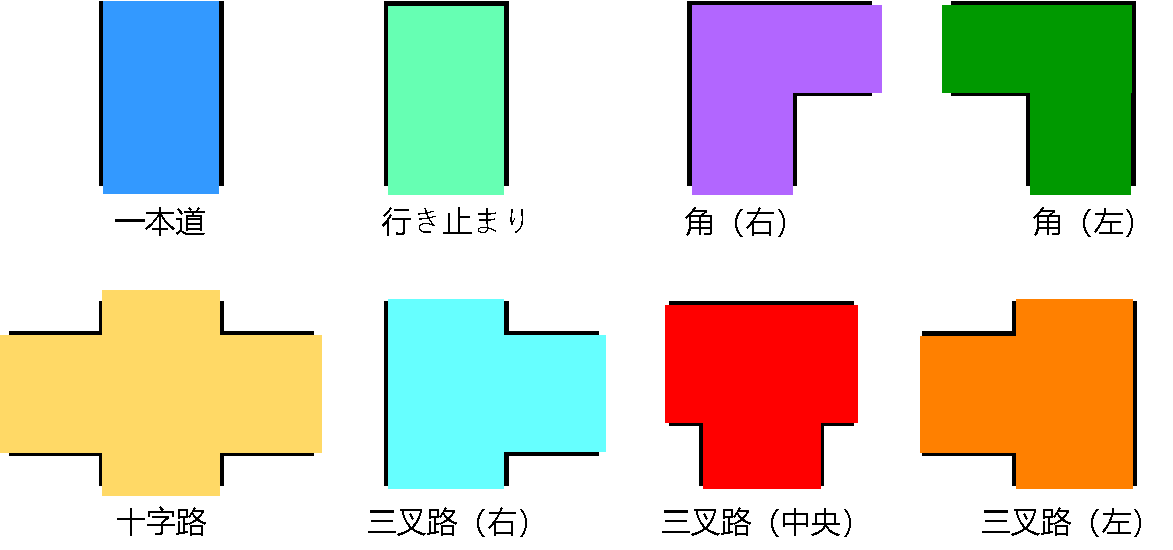
\includegraphics[width=100mm]{images/pdf/class.pdf}
     \caption{Path-following module system Quoted from \cite{haruyama2023}}
     \label{fig:class}
\end{figure}
\newpage

ネットワークの構成を\ref{fig:int_net}に示す.
このネットワークアーキテクチャはDhaivat らが提案するCNNとLSTMを組み合わせた
IntersectNet[7] に倣って構築した.
なおCNNアーキテクチャは実時間性の観点からAlexNetからMovileNetV3-Largeへ変更している.

ネットワークはフレーム数 16,画像サイズ64×48の連続したRGB画像データを入力とする.
画像データは各フレームごとにCNNで処理され,この特徴ベクトルはLSTMへ入力される.
各LSTMの出力は分類層(全結合層)へ渡される.
最後に,全ての分類層の出力を融合層へ渡し,融合層は入力の平均を取ることで,
最終的な分類結果を出力する.
損失関数としてCrossEntropyLoss,活性化関数にはAdamを使用する.
\begin{figure}[htbp]
    \centering
     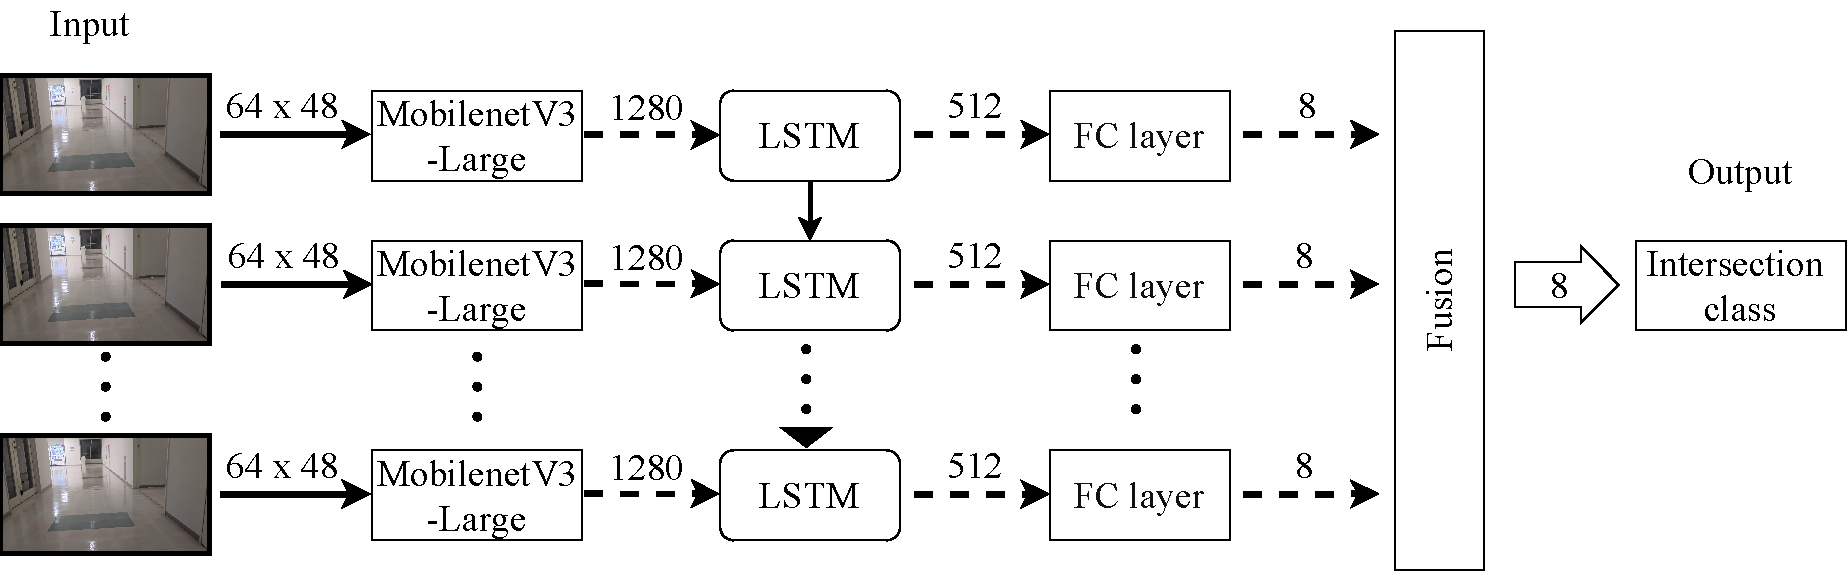
\includegraphics[width=120mm]{images/pdf/network-intersect.pdf}
     \caption{Path-following module system}
     \label{fig:int_net}
\end{figure}

次に通路分類モジュールのデータセットの作成について述べる.
データの作成では,経路追従モジュールの学習と同様に,
メトリックマップに基づいたルールベース制御器によって経路を走行する.
その際,フレーム数 16 の連続したカメラ画像と通路の分類ラベルを1組とし,
0.125秒周期でデータセットへ加える.分類ラベルのアノテーションは,
\ref{fig:int_net}に示すように,通路の特徴を予めメトリックマップに登録しておくことで,自動的に行う.
\begin{figure}[htbp]
    \centering
     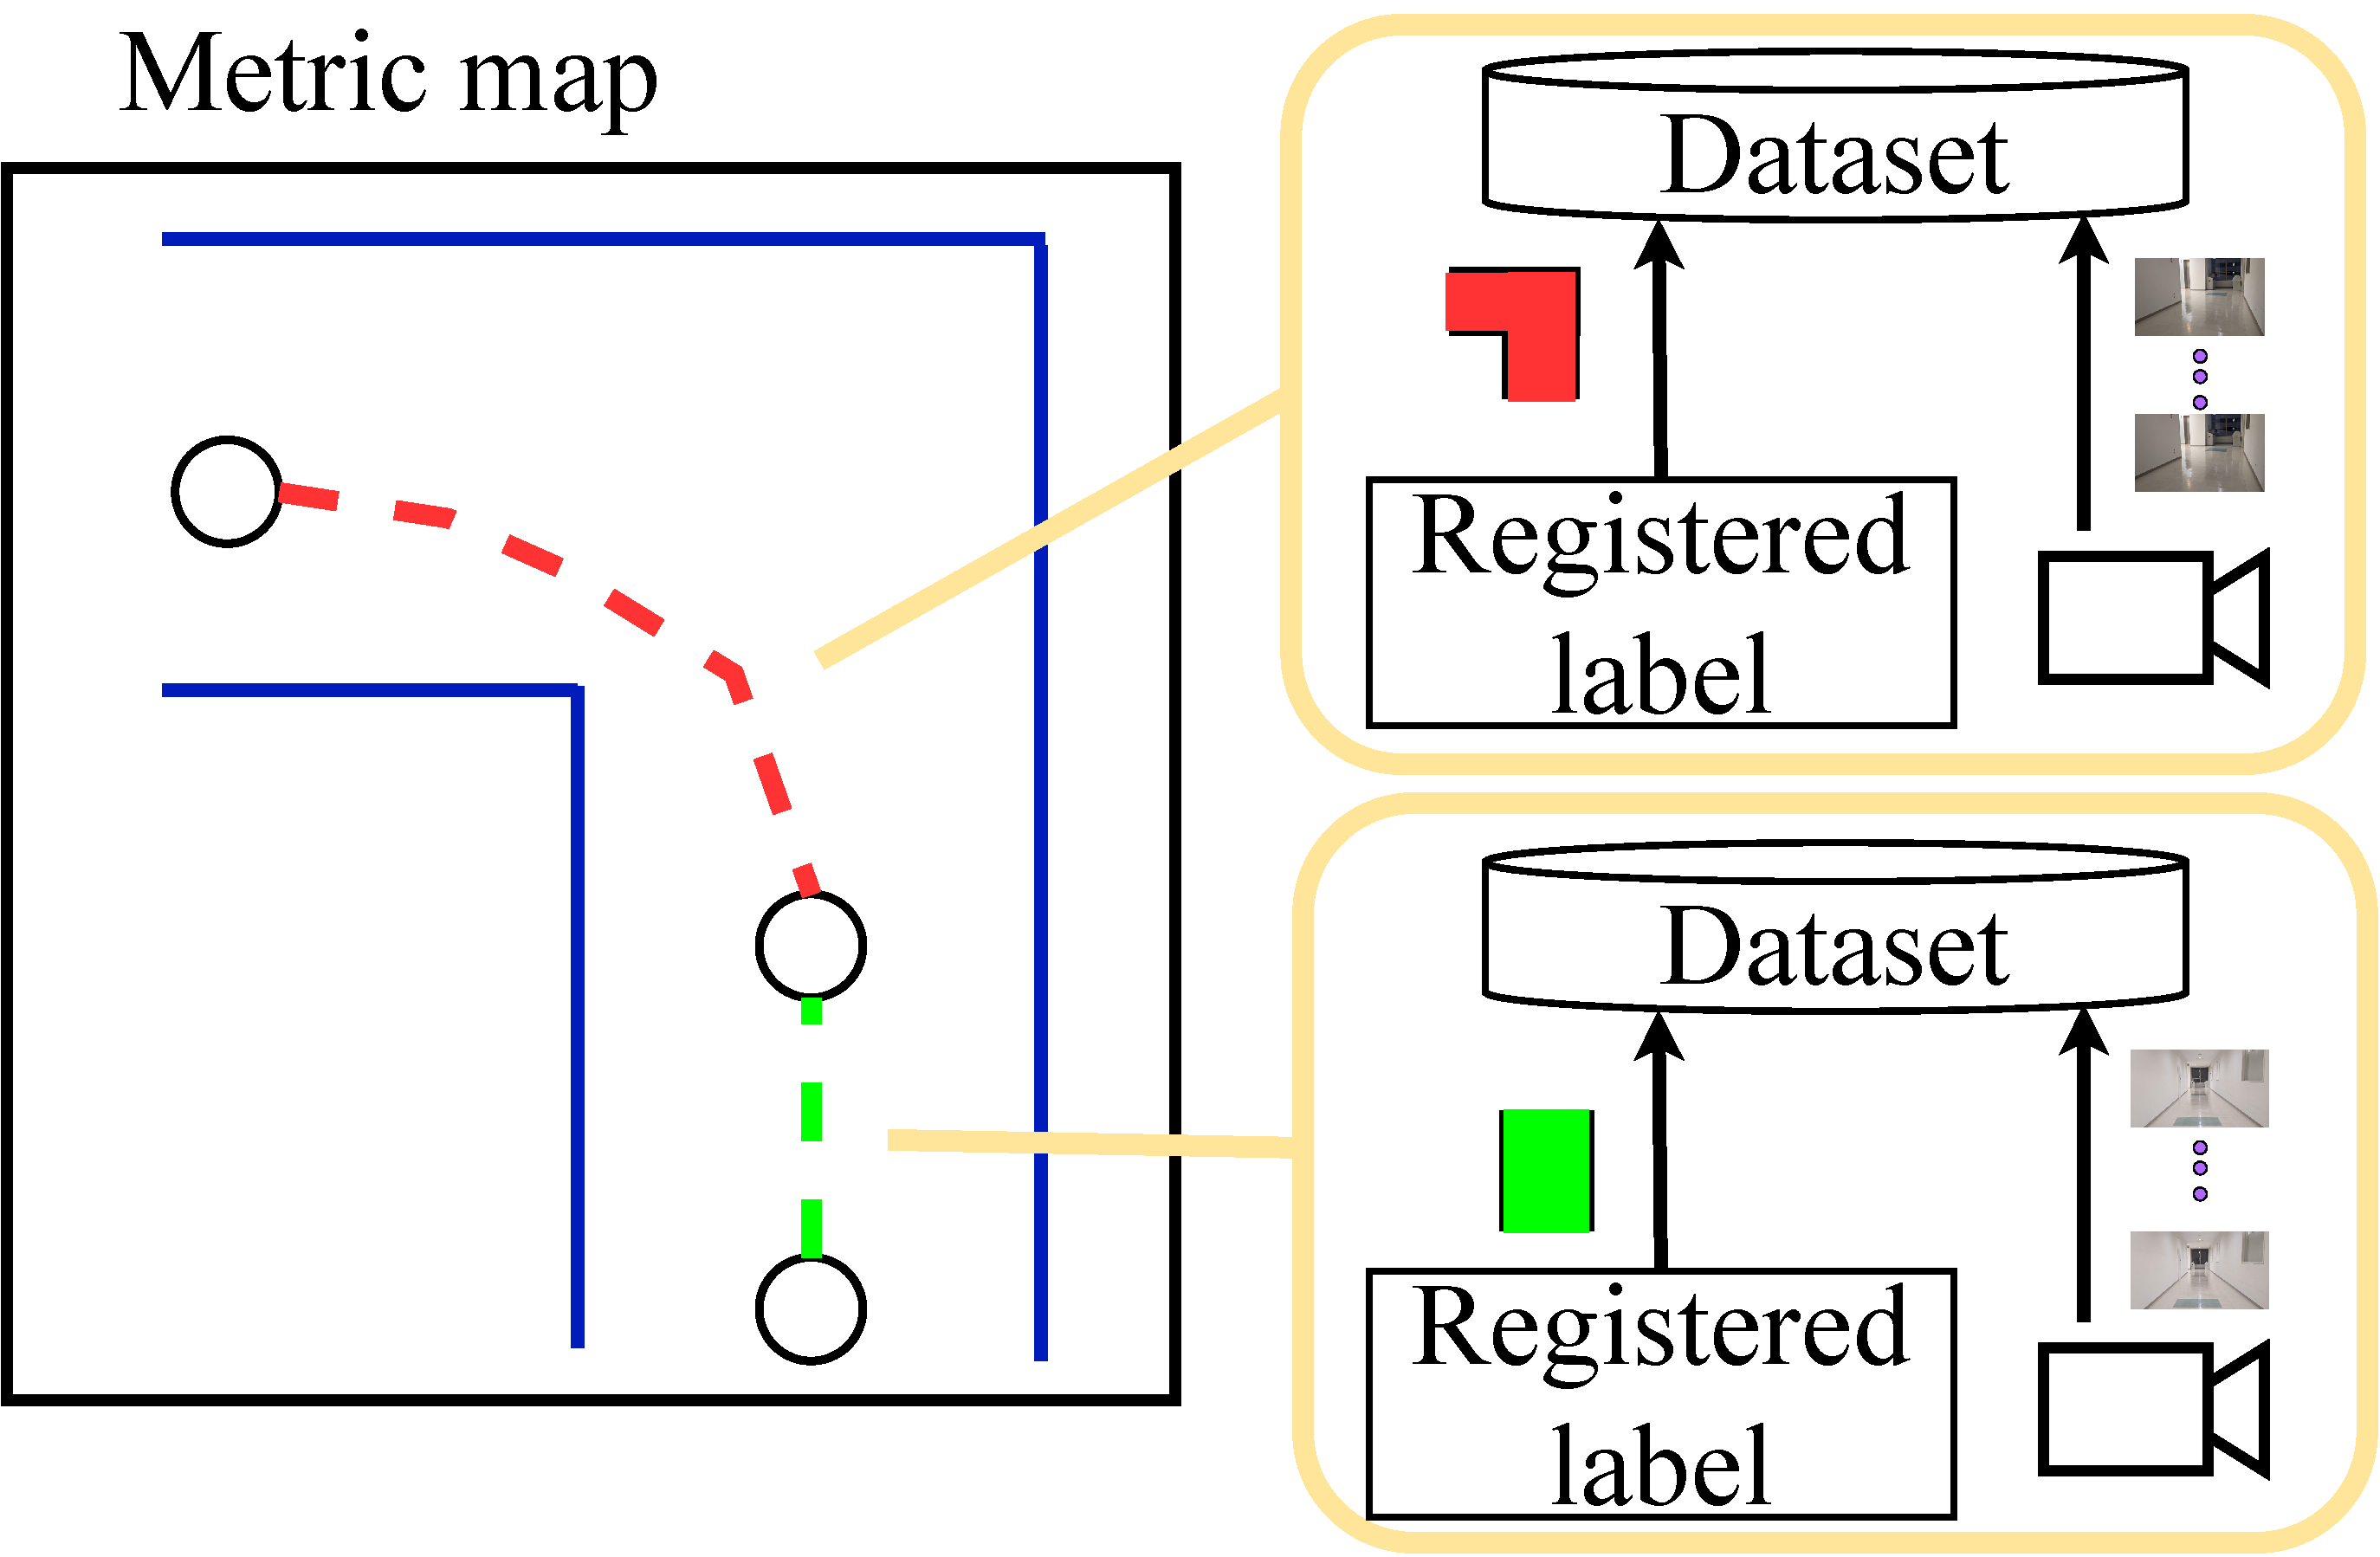
\includegraphics[width=100mm]{images/pdf/map_label.pdf}
     \caption{Path-following module system}
     \label{fig:int_net}
\end{figure}
\newpage
学習するデータセット内で,各クラスのデータ数か
大きく異なる不均衡データは,分類結果に大きな影響を与える
とされている. 経路追従モジュールではオーバーサンプリングを行ったが,
そのため,本稿では学習する際に,
データセット内のクラス間のデータ数によって重
み付けを行うコストアプローチを導入している.
具体的には,損失関数である損失関数(CrossEntropyLoss)で用いる
クラスごとの重みをメジャーデータを基に決定する.